\documentclass[a4paper,10pt,titlepage]{article}
\usepackage[portuguese]{babel}
\usepackage[utf8]{inputenc}
\usepackage[ruled,linesnumbered]{algorithm2e}
\usepackage[table,xcdraw]{xcolor}
\newcommand{\HRule}{\rule{\linewidth}{0.5mm}}
\usepackage{graphics} 
\usepackage{epsfig} 
\usepackage{amsmath} 
\usepackage{amssymb}  
\usepackage{nicefrac}
\usepackage{subfig}
\usepackage{setspace}
\usepackage{microtype}
\usepackage{color}
\usepackage{amsthm}
\usepackage{listings,xcolor}
\usepackage{ragged2e}
\usepackage{times}
\usepackage{multicol}
\usepackage{tabularx}
\usepackage{geometry}
\geometry{
 a4paper,
 total={170mm,257mm},
 left=20mm,
 top=20mm,
 }

\begin{document} 

%--------------------> CAPA <-----------------------
\begin{titlepage}
    \begin{justify}
        \begin{center}
            \begin{large} 
                NOME COMPLETO DA ORGANIZAÇÃO\\[1.5cm]
                \textbf{CURSO}\\[0.5cm]
                \textbf{PROJETO}\\[3cm]
                \textbf{TEMA}\\[6cm]
            
                NOME DO(A) ALUNO(A)\vfill
            
                Cidade\\[0.5cm]
                Ano\\
            \end{large}
        \end{center}
    \end{justify}
\end{titlepage}


\begin{titlepage}
    \begin{justify}
        \begin{center}
            \begin{large} 
                NOME COMPLETO DA ORGANIZAÇÃO\\[1.5cm]
                \textbf{CURSO}\\[0.5cm]
                \textbf{PROJETO}\\[3cm]
                \textbf{TEMA}\\[6cm]
            
                \hspace{.45\textwidth}
                
        \begin{flushright}        
            \begin{minipage}{.5\textwidth} 
                Produção apresentada ao (Instituição de (Cidade), como exigência parcial para carga horária do (Curso), sob orientação do(a) Orientador(a) (Nome).
            \end{minipage}
        \end{flushright}\vfill 
        
                Cidade\\[0.5cm]
                Ano\\
            \end{large}
        \end{center}
    \end{justify}
\end{titlepage}

%-------------------> RESUMO <----------------------
\begin{center}
    \begin{Large}
        RESUMO
    \end{Large}
\end{center}

\begin{onehalfspacing}
    \begin{justify}
        \begin{large}
            Este projeto teve por componente principal a ampliação de conhecimentos relacionados ao (tema) em empresas de fornecimento de soluções de (tema). Pesquisas teóricas sobre os norteadores de uma empresa, bem como sua estrutura organizacional, sua infraestrutura de TI e seus serviços foram responsáveis por estruturar essa primeira parte do projeto. Ao final da pesquisa, foi definida uma empresa de fornecimento de soluções de (tema) para visita futura, afim de compreender sua missão, visão e valores, assim como sua estrutura organizacional.
        \end{large}
    \end{justify}
\end{onehalfspacing}
    
\begin{onehalfspacing}
    \begin{justify}
        \begin{large}
            \textbf{Palavras-chave:} 1. Tema. 2. Tema. 3. Estrutura Organizacional. 4. Tema. 5. Tema.
            \end{large}
        \end{justify}
\end{onehalfspacing}\pagebreak

%------------------> ABSTRACT <--------------------
\begin{center}
    \begin{Large}
        ABSTRACT
    \end{Large}
\end{center}

\begin{onehalfspacing}    
    \begin{justify}
        \begin{large}
            This project had as main component the expansion of knowledge related to (topic) . Theoretical research about the guidelines of a company, as well as it's organizational structure, IT infrastructure and services were responsible for structuring this first part of the project. At the end of the research, an (topic) company was defined for a future visit, in order to understand your mission, vision and values, as well as your organizational structure.
        \end{large}
    \end{justify}
\end{onehalfspacing}
    
\begin{onehalfspacing} 
    \begin{justify}
        \begin{large}
                \textbf{Keywords:} 1. Topic. 2. Topic. 3. Topic. 4. Topic. 5. Topic.
        \end{large}
    \end{justify}
\end{onehalfspacing}\pagebreak

%--------------------> LISTAS <----------------------
\begin{doublespacing}
    \begin{center}
        \begin{large}
            \listoffigures
        \end{large}
    \end{center}
\end{doublespacing}\pagebreak

\begin{doublespacing}
    \begin{center}
        \begin{large}
            \listoftables
        \end{large}
    \end{center}
\end{doublespacing}\pagebreak

\begin{onehalfspacing}
    \begin{center}
        \begin{large}
            \tableofcontents
        \end{large}
    \end{center}
\end{onehalfspacing}\pagebreak

%--------------------> INPUTS <----------------------
    \section{INTRODUÇÃO}\label{sec:intro}
    \subsection{Tema}

\begin{onehalfspacing}
    \begin{justify}
        \begin{large}
            Texto. Texto. Texto. Texto. Texto. Texto. Texto. Texto. Texto. Texto. Texto. Texto. Texto. Texto. Texto. Texto. Texto. Texto. Texto. Texto. Texto. Texto. Texto. Texto. Texto. Texto. Texto. Texto. Texto. Texto. Texto. Texto. Texto. Texto. Texto. Texto. Texto. Texto. Texto. Texto. Texto. Texto. Texto. Texto. Texto. Texto. Texto. Texto. Texto. Texto. Texto. Texto. Texto. Texto. Texto. Texto. Texto. Texto. Texto. Texto. Texto. Texto. Texto. Texto. Texto. Texto. Texto. Texto. Texto. Texto. Texto. Texto. Texto. Texto. Texto. Texto. Texto. Texto. Texto. Texto. Texto. Texto. Texto. Texto. Texto. Texto. Texto. Texto. Texto. Texto. Texto. Texto. Texto. Texto. Texto. Texto. Texto. Texto. Texto. Texto. Texto. Texto. Texto. Texto. Texto. Texto. Texto. Texto. Texto. Texto. Texto. Texto. Texto. Texto. Texto. Texto. Texto. Texto. Texto. Texto. Texto. Texto. Texto. Texto. Texto. Texto. Texto. Texto. Texto. Texto. Texto. Texto. Texto. Texto. Texto. Texto.
        \end{large}
    \end{justify}
\end{onehalfspacing}

\begin{figure}[ht]\caption{Gráfico - Relatório de Vacância}
    \centering
        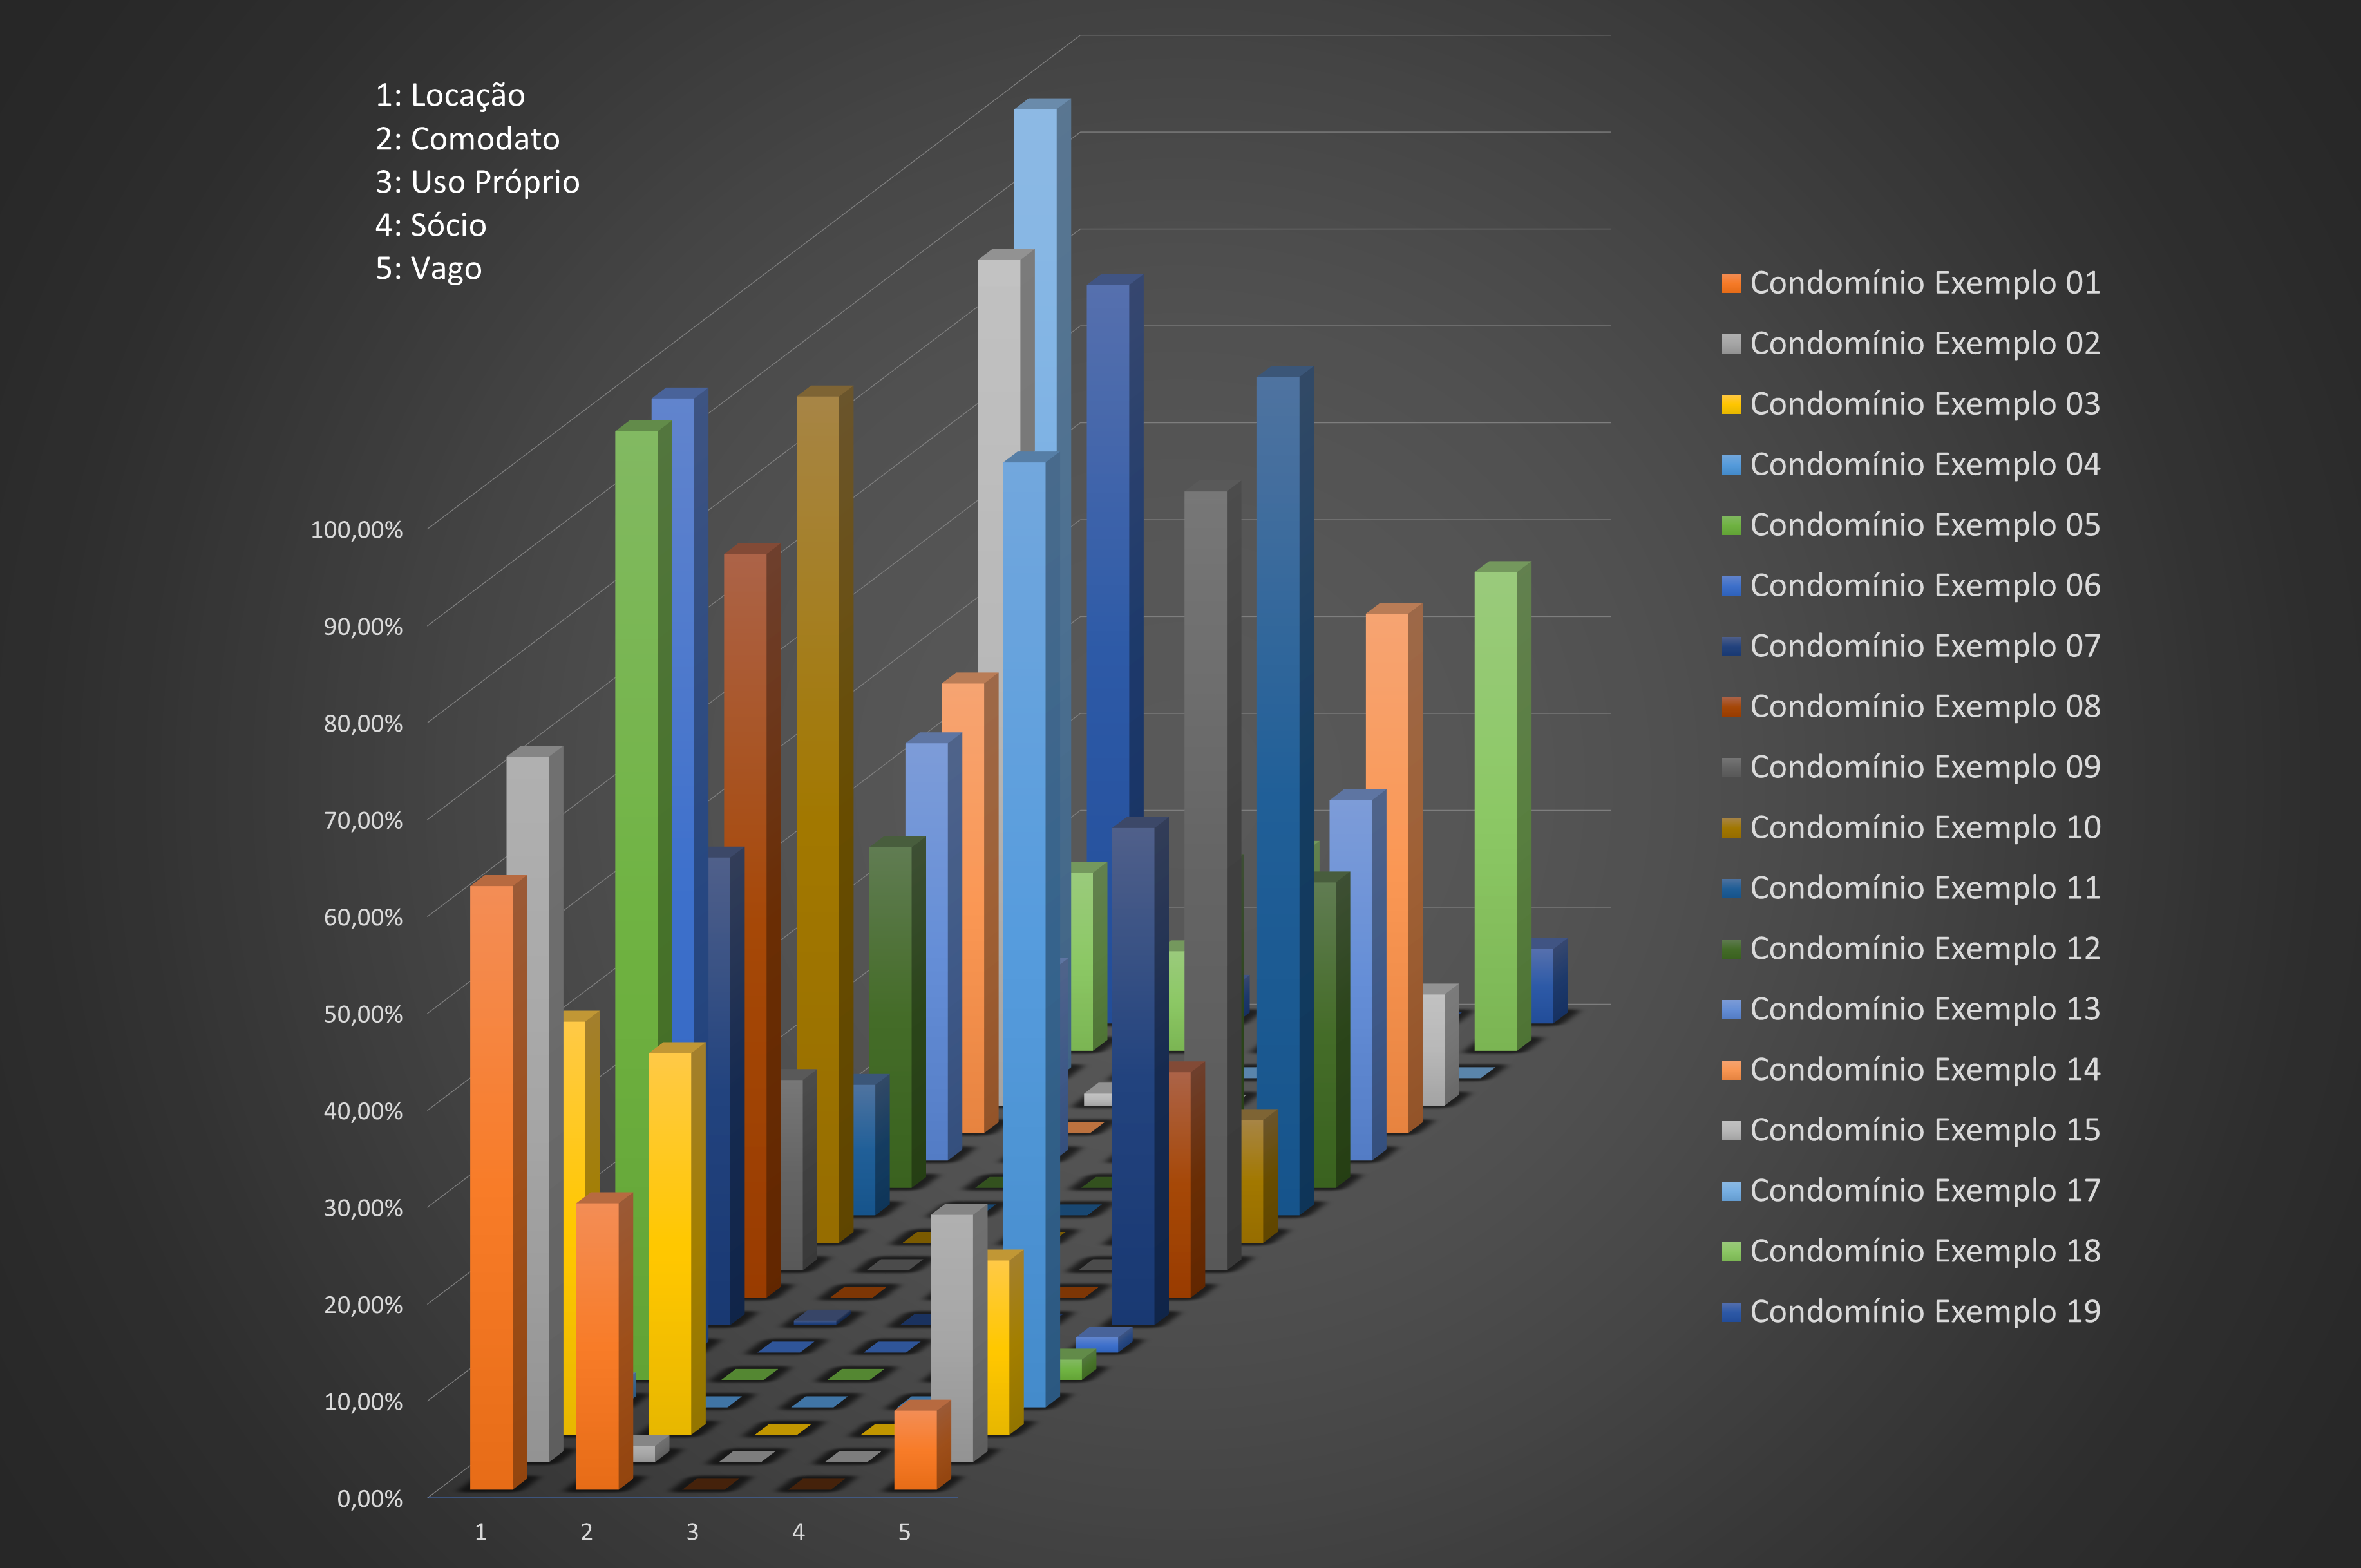
\includegraphics[scale = 0.5]{images/relatorio-vacancia.png}
        \label{figure:tiposdeinovacao}
\end{figure}
\begin{flushleft}
    \begin{small}
        Fonte: adaptado de Vitória Peçanha de Araújo (2021).\\
    \end{small}
\end{flushleft}

\begin{onehalfspacing}
    \begin{justify}
        \begin{large}
            Texto. Texto. Texto. Texto. Texto. Texto. Texto. Texto. Texto. Texto. Texto. Texto. Texto. Texto. Texto. Texto. Texto. Texto. Texto. Texto. Texto. Texto. Texto. Texto. Texto. Texto. Texto. Texto. Texto. Texto. Texto. Texto. Texto. Texto. Texto. Texto. Texto. Texto. Texto. Texto. Texto. Texto. Texto. Texto. Texto. Texto. Texto. Texto. Texto. Texto. Texto. Texto. Texto. Texto. Texto. Texto. Texto. Texto. Texto. Texto. Texto. Texto. Texto. Texto. Texto. Texto. Texto. Texto. Texto. Texto. Texto. Texto. Texto. Texto. Texto. Texto. Texto. Texto. Texto. Texto. Texto. Texto. Texto. Texto. Texto. Texto. Texto. Texto. Texto. Texto. Texto. Texto. Texto. Texto. Texto. Texto. Texto. Texto. Texto. Texto. Texto. Texto. Texto. Texto. Texto. Texto. Texto. Texto. Texto. Texto. Texto. Texto. Texto. Texto. Texto. Texto. Texto. Texto. Texto. Texto. Texto. Texto. Texto. Texto. Texto. Texto. Texto. Texto. Texto. Texto. Texto. Texto. Texto. Texto. Texto.
        \end{large}
    \end{justify}
\end{onehalfspacing}\pagebreak

%----------------> JUSTIFICATIVA <-------------------
    \subsection{Justificativa}
    
\begin{onehalfspacing}
    \begin{justify}
        \begin{large}
            Texto. Texto. Texto. Texto. Texto. Texto. Texto. Texto. Texto. Texto. Texto. Texto. Texto. Texto. Texto. Texto. Texto. Texto. Texto. Texto. Texto. Texto. Texto. Texto. Texto. Texto. Texto. Texto. Texto. Texto. Texto. Texto. Texto. Texto. Texto. Texto. Texto. Texto. Texto. Texto. Texto. Texto. Texto. Texto. Texto. Texto. Texto. Texto. Texto. Texto. Texto. Texto. Texto. Texto. Texto. Texto. Texto. Texto. Texto. Texto. Texto. Texto. Texto. Texto. Texto. Texto. Texto. Texto. Texto. Texto. Texto. Texto. Texto. Texto. Texto. Texto. Texto. Texto. Texto. Texto. Texto. Texto. Texto. Texto. Texto. Texto. Texto. Texto. Texto. Texto. Texto. Texto. Texto. Texto. Texto. Texto. Texto. Texto. Texto. Texto. Texto. Texto. Texto. Texto. Texto. Texto. Texto. Texto. Texto. Texto. Texto. Texto. Texto. Texto. Texto. Texto. Texto. Texto. Texto. Texto. Texto. Texto. Texto. Texto. Texto. Texto. Texto. Texto. Texto. Texto. Texto. Texto. Texto. Texto. Texto.
        \end{large}
    \end{justify}
\end{onehalfspacing}

%------------------> OBJETIVOS <---------------------
    \subsection{Objetivos}

\begin{onehalfspacing}
    \begin{justify}
        \begin{large}
            Texto. Texto. Texto. Texto. Texto. Texto. Texto. Texto. Texto. Texto. Texto. Texto. Texto. Texto. Texto. Texto. Texto. Texto. Texto. Texto. Texto. Texto. Texto. Texto. Texto. Texto. Texto. Texto. Texto. Texto. Texto. Texto. Texto. Texto. Texto. Texto. Texto. Texto. Texto. Texto. Texto. Texto. Texto. Texto. Texto. Texto. Texto. Texto. Texto. Texto. Texto. Texto. Texto. Texto. Texto. Texto. Texto. Texto. Texto. Texto. Texto. Texto. Texto. Texto. Texto. Texto. Texto. Texto. Texto. Texto. Texto. Texto. Texto. Texto. Texto. Texto. Texto. Texto. Texto. Texto. Texto. Texto. Texto. Texto. Texto. Texto.
        \end{large}
    \end{justify}
\end{onehalfspacing}

%------------------> TABELA 1 <---------------------
\begin{onehalfspacing}
    \renewcommand\tabularxcolumn[1]{>{\Centering}m{#1}} 
        \begin{table}[ht]
        \caption{Tabela de exemplo de tema}
            \begin{center}\large
                \begin{tabularx}{\textwidth}{|X|X|}
                    \hline
                    \textbf{Texto 1} \cellcolor{black!20} & \textbf{Texto 2} \cellcolor{black!20}  \\
                    \hline
                    Texto. Texto. Texto. Texto. Texto. Texto. Texto. Texto. Texto. \cellcolor{black!5} & \textbf{Texto 3}
                        
                    Descrição, descrição, descrição
                    
                    \textbf{Texto 4}
                        
                    Descrição - Descrição
                    Descrição - Descrição

                    \textbf{Texto 5}
                        
                    Dados - Dados, dados
                        
                    Dados - Dados, dados

                    \textbf{Texto 6}
                        
                    000×000

                    \textbf{Texto 7}
                        
                    Descrição, descrição, descrição AAAA 1.0 \cellcolor{black!5} \\
                \hline
            \end{tabularx}
        \end{center}
        \begin{small}
            Fonte: adaptado de Autor (2021).\\
        \end{small}
    \end{table}
\end{onehalfspacing}

\begin{onehalfspacing}
    \begin{justify}
        \begin{large}
            Texto. Texto. Texto. Texto. Texto. Texto. Texto. Texto. Texto. Texto. Texto. Texto. Texto. Texto. Texto. Texto. Texto. Texto. Texto. Texto. Texto. Texto. Texto. Texto. Texto. Texto. Texto. Texto. Texto.
        \end{large}
    \end{justify}
\end{onehalfspacing}\pagebreak





    \section{RELATÓRIO}\label{sec:report}
    \subsection{Tema}

\begin{onehalfspacing}
    \begin{justify}
        \begin{large}
            Texto\cite{livro-qualquer}. Texto. Texto. Texto. Texto. Texto. Texto. Texto. Texto. Texto. Texto. Texto. Texto. Texto. Texto. Texto. Texto. Texto\cite{artigo-de-economia}. Texto. Texto. Texto. Texto. Texto. Texto. Texto. Texto. Texto. Texto. Texto. Texto. Texto. Texto. Texto. Texto. Texto. Texto. Texto. Texto. Texto. Texto. Texto. Texto. Texto. Texto. Texto. Texto. Texto. Texto. Texto. Texto. Texto. Texto. Texto. Texto. Texto. Texto. Texto. Texto. Texto. Texto. Texto. Texto. Texto. Texto. Texto. Texto. Texto. Texto. Texto. Texto. Texto. Texto. Texto. Texto. Texto. Texto. Texto. Texto. Texto. Texto. Texto. Texto. Texto. Texto. Texto. Texto. Texto. Texto. Texto. Texto. Texto. Texto. Texto. Texto. Texto. Texto. Texto. Texto. Texto. Texto. Texto. Texto. Texto. Texto. Texto. Texto. Texto. Texto. Texto. Texto. Texto. Texto. Texto. Texto. Texto. Texto. Texto. Texto. Texto. Texto. Texto. Texto. Texto. Texto. Texto. Texto. Texto. Texto. Texto. Texto. Texto. Texto. Texto. Texto. Texto\footnote[1]{Definição do texto anexado na nota de rodapé.}:
        \end{large}
    \end{justify}
\end{onehalfspacing}

%-------------------> TABELA 2 <----------------------
\begin{onehalfspacing}
    \renewcommand\tabularxcolumn[1]{>{\Centering}m{#1}} 
    \begin{table}[ht]
        \begin{center}
            \begin{large}
                \caption{Tema 01}
                \begin{tabular}{r|lr}
                    \hline
                    \textbf{Título 1} & \textbf{Título 2} \\
                    \hline
                    Definição & Descrição, descrição \\
                    Descrição & Definição   \\
                    \hline
                \end{tabular}
            \end{large}
        \end{center}
   \end{table}
\end{onehalfspacing}

%-------------------> TABELA 3 <----------------------
\begin{onehalfspacing}
    \renewcommand\tabularxcolumn[1]{>{\Centering}m{#1}} 
    \begin{table}[ht]
        \begin{center}
            \begin{large}
                \caption{Tema 02}
                \begin{tabular}{r|lr}
                    \hline
                    \textbf{Título 3} & \textbf{Título 4} \\
                    \hline
                    Descrição, descrição & Definição, definição \\
                    Tópico, Tópico & Temática, temática \\
                    Descrição, descrição & Definição, definição   \\
                    Tópico, Tópico & Temática, temática \\
                    Descrição, descrição & Definição, definição \\
                    Tópico, Tópico & Temática, temática   \\
                    Descrição, descrição & Definição, definição \\
                    \hline
                \end{tabular}
            \end{large}
        \end{center}
            \begin{small}
                Fonte: adaptado de Autor (2021).
            \end{small}
        \end{table}
\end{onehalfspacing}

\begin{onehalfspacing}
    \begin{justify}
        \begin{large}
            Texto. Texto. Texto. Texto. Texto. Texto. Texto. Texto. Texto. Texto. Texto. Texto. Texto. Texto. Texto. Texto. Texto. Texto. Texto. Texto. Texto. Texto. Texto. Texto. Texto. Texto. Texto. Texto. Texto. Texto. Texto. Texto. Texto. Texto. Texto. Texto. Texto. Texto. Texto. Texto. Texto. Texto. Texto. Texto. Texto. Texto. Texto. Texto. Texto. Texto. Texto. Texto. Texto. Texto. Texto. Texto. Texto. Texto. Texto. Texto. Texto. Texto. Texto. Texto. Texto. Texto. Texto. Texto. Texto. Texto. Texto. Texto. Texto. Texto. Texto. Texto. Texto. Texto. Texto. Texto. Texto. Texto. Texto. Texto. Texto. Texto. Texto. Texto. Texto. Texto. Texto. Texto. Texto. Texto. Texto. Texto. Texto. Texto. Texto. Texto. Texto. Texto. Texto. Texto. Texto. Texto. Texto. Texto. Texto. Texto. Texto. Texto. Texto. Texto. Texto. Texto. Texto. Texto. Texto. Texto. Texto. Texto. Texto. Texto. Texto. Texto. Texto. Texto. Texto. Texto. Texto. Texto. Texto. Texto. Texto.\vfill
        \end{large}
    \end{justify}
\end{onehalfspacing}\pagebreak
    \section{CONSIDERAÇÕES FINAIS}\label{sec:conclusion}

\begin{onehalfspacing}
    \begin{justify}
        \begin{large}
            \noindent Texto. Texto. Texto. Texto. Texto. Texto. Texto. Texto. Texto. Texto. Texto. Texto. Texto. Texto. Texto. Texto. Texto. Texto. Texto. Texto. Texto. Texto. Texto. Texto. Texto. Texto. Texto. Texto. Texto. Texto. Texto. Texto. Texto. Texto. Texto. Texto. Texto. Texto. Texto. Texto. Texto. Texto. Texto. Texto. Texto. Texto. Texto. Texto. Texto. Texto. Texto. Texto. Texto. Texto. Texto. Texto. Texto. Texto. Texto. Texto. Texto. Texto. Texto. Texto. Texto. Texto. Texto. Texto. Texto. Texto. Texto. Texto. Texto. Texto. Texto. Texto. Texto. Texto. Texto. Texto. Texto. Texto. Texto. Texto. Texto. Texto. Texto. Texto. Texto. Texto. Texto. Texto. Texto. Texto. Texto. Texto. Texto. Texto. Texto. Texto. Texto. Texto. Texto. Texto. Texto. Texto. Texto. Texto. Texto. Texto. Texto. Texto. Texto. Texto. Texto. Texto. Texto. Texto. Texto. Texto. Texto. Texto. Texto. Texto. Texto. Texto. Texto. Texto. Texto. Texto. Texto. Texto. Texto. Texto.\\
            
            \noindent No entanto, este é um resumo do pensamento do autor, como de acordo com Autor (2021):\\
        \end{large}
    \end{justify}
\end{onehalfspacing}

\begin{onehalfspacing}               
    \begin{center}\hspace{.20\textwidth}
        \begin{minipage}{.60\textwidth}
            \begin{small}
                Esta é uma citação direta. Esta é uma citação direta. Esta é uma citação direta. Esta é uma citação direta. Esta é uma citação direta. Esta é uma citação direta. Esta é uma citação direta. Esta é uma citação direta. Esta é uma citação direta. Esta é uma citação direta. Esta é uma citação direta. Esta é uma citação direta. Esta é uma citação direta. (AUTOR, 2021)\\
            \end{small}
        \end{minipage}
    \end{center}
\end{onehalfspacing}

\pagebreak


    
%-----------------> BIBLIOGRAFIA <-------------------
\begin{onehalfspacing}
    \begin{center}
        \begin{large}
            \bibliographystyle{alpha}
            \bibliography{references}
        \end{large}
    \end{center}
\end{onehalfspacing}
    
\end{document}
